\begin{frame} \frametitle{The Block-chain database} 
	\begin{center}
		As database for new faces, we implemented a \textbf{Block-chain}. \\ 
		We used an open-source implementation of it, called 
		BigchainDB\footnote{Main page: {\color{red} 
		\url{https://www.bigchaindb.com}}. Documentation {\color{red}
		\href{http://docs.bigchaindb.com/projects/server/en/latest/introduction.html}
		{here}}.}. \\ We also used Docker\footnote{Main page: {\color{red} 
		\url{https://www.docker.com}}.} to deploy 4 containers running the
		application.
	\end{center}
	\vfill
	\begin{minipage}{.45\textwidth}
		\begin{figure}[H]
			
\includegraphics[width=.8\textwidth]{img/bchaindb}
		\end{figure}
	\end{minipage}
	\hfill
	\begin{minipage}{.45\textwidth}
		\begin{figure}[H]
			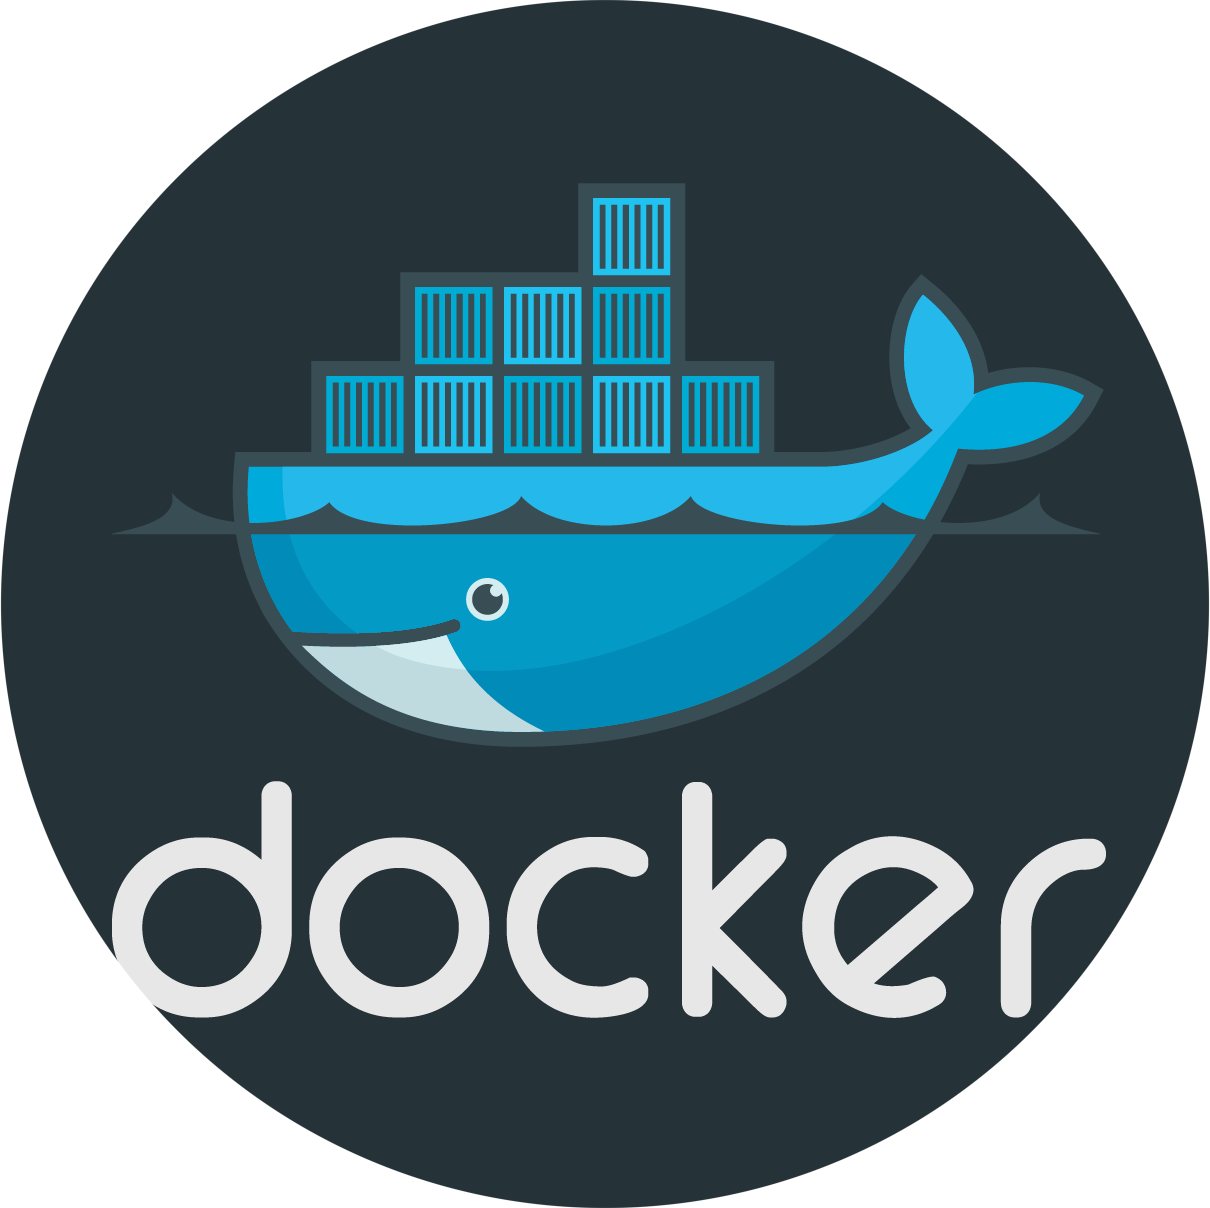
\includegraphics[width=.8\textwidth]{img/dockerlogo}
		\end{figure}
	\end{minipage}
	\vfill
\end{frame}
	
\begin{frame} \frametitle{Architecture Implementation\footnote{This is absolutely not meant for a real deployment!!}}
	\begin{center} \begin{tikzpicture}[
		container/.style={rectangle, draw=black, fill=cyan!5 ,very thick, 
		minimum size=0.3in, align=center},
		ports/.style={draw=black, thick, rectangle, rounded corners=1.5ex,
		minimum height=0.2in, minimum width=1.5in,align=center, rotate=90}
	]
		
		% Bigchaindb dockers
		\node[container, label={above:\footnotesize node1.com}] 
		(1) at (1,3.5) 
		{\scriptsize Container: \\ \scriptsize \color{blue} Bigchain DB\#1};
		\node[container, label={above:\footnotesize node2.com}] 
		(2) at (3.5,3.5) 
		{\scriptsize Container: \\ \scriptsize \color{blue} Bigchain DB\#2};
		\node[container, label={below:\footnotesize node3.com}] 
		(3) at (1,1) 
		{\scriptsize Container: \\ \scriptsize \color{blue} Bigchain DB\#3};
		\node[container, label={below:\footnotesize node4.com}] 
		(4) at (3.5,1) 
		{\scriptsize Container: \\ \scriptsize \color{blue} Bigchain DB\#4};
		
		% Nginx container
		\node[container] 
		(5) at (4.8,2.25) {\scriptsize Container: \\ \scriptsize \color{red} Nginx};
			
		% Ports
		\node[ports] (6) at (6.5,2.25) {\scriptsize Docker Ports};
		\node[ports] (7) at (8.5,2.25) {\scriptsize Server Ports};
			
		% Outline Boxes	
		\node(n1)[draw, blue, very thick, fit=(1)(2)(3)(4)(5)(6), 
		inner sep=0.15in, label={above:\footnotesize DOCKER SETUP}]{};
		\node(n2)[draw, brown, very thick, fit=(n1)(7),
		inner sep=0.2in,label={above:\footnotesize PHISICAL SERVER}]{};
			
		% Containers to Nginx	
		\draw[<->] (1.south) .. controls + (down:0.5em) .. ([yshift=0.25em]5.west);
		\draw[<->] (2.south) .. controls + (down:0.35em) .. ([yshift=0.75em]5.west);
		\draw[<->] (3.north) .. controls + (up:0.5em) .. ([yshift=-0.25em]5.west);
		\draw[<->] (4.north) .. controls + (up:0.35em) .. ([yshift=-0.75em]5.west);
	
		% Nginx to docker ports			
		\draw[very thick,<->,blue!30] (5.east) -- (6.north);
				
		% docker ports to server ports	
		\draw[thick, red, <->] ([yshift=0.6in]6.south) -- 
		node[above]{\parbox[t]{2em}
		{\centering \tiny 22:22}} ([yshift=0.6in]7.north);
			
		\draw[thick, red, <->] ([yshift=0.45in]6.south) -- 
		node[above]{\parbox[t]{2em}
		{\centering \tiny 80:80}} ([yshift=0.45in]7.north);
		
		\draw[thick, red, <->] ([yshift=0.3in]6.south) -- 
		node[above]{\parbox[t]{3em}
		{\centering \tiny 443:443}} ([yshift=0.3in]7.north);
			
		\draw[thick, red, <->] ([yshift=0.15in]6.south) -- 
		node[above]{\parbox[t]{4em}
		{\centering \tiny 9984:9984}} ([yshift=0.15in]7.north);
	
		\draw[thick, red, <->] (6.south) -- 
		node[above]{\parbox[t]{4em}
		{\centering \tiny 9985:9985}} (7.north);
				
		\draw[thick, red, <->] ([yshift=-0.15in]6.south) -- 
		node[above]{\parbox[t]{4em}
		{\centering \tiny 2812:2812}} ([yshift=-0.15in]7.north);
				
		\draw[thick, red, <->] ([yshift=-0.3in]6.south) -- 
		node[above]{\parbox[t]{5em}
		{\centering \tiny 26656:26656}} ([yshift=-0.3in]7.north);
				
		\draw[thick, red, <->] ([yshift=-0.45in]6.south) -- 
		node[above]{\parbox[t]{5em}
		{\centering \tiny 26657:26657}} ([yshift=-0.45in]7.north);
			
		\draw[thick, red, <->] ([yshift=-0.6in]6.south) -- 
		node[above]{\parbox[t]{5em}
		{\centering \tiny 27017:27017}} ([yshift=-0.6in]7.north);
	\end{tikzpicture} \end{center}
\end{frame}
		
\begin{frame} \frametitle{How to interact with the DB}
	We are assuming that we have an enstablished connection set up.
	\vfill
	\begin{block}{Query data}
		\texttt{connection.searchAssets('AwesomeAsset') \\
		.then(assets =$>$ console.log('Found assets:', assets))\\
		// Read the console to look at the assets}
	\end{block}
	\vfill
	\begin{block}{Load data (make a transaction)}
		\texttt{// Create transaction first (txTransferBob)				
		driver.Transaction.signTransaction(txTransferBob, alice.privateKey);	
		\\conn.postTransactionCommit(txTransferBobSigned);}
	\end{block}
	\vfill
	Simple as that...
\end{frame}